\حصہء{سوالات}
سوال \حوالہ{سوال_سمتیہ_غیر_سمتی_الف} تا سوال \حوالہ{سوال_سمتیہ_غیر_سمتی_ب} میں درج ذیل دریافت کریں۔
\begin{enumerate}[a.]
\item
\عددی{\kvec{A}\cdot\kvec{B}}، \عددی{\abs{\kvec{A}}}، \عددی{\abs{\kvec{B}}}
\item
\عددی{\kvec{A}} اور \عددی{\kvec{B}} کے بیچ زاویہ کا کوسائن۔
\item
\عددی{\kvec{A}} کے رخ \عددی{\kvec{B}} کا غیر سمتی جزو۔
\item
سمتیہ \عددی{\proj_{\kvec{A}}\,\kvec{B}}
\end{enumerate}

\ابتدا{سوال}\شناخت{سوال_سمتیہ_غیر_سمتی_الف}
$\kvec{A}=2\ai-4\aj+\sqrt{5}\ak,\quad \kvec{B}=-2\ai+4\aj-\sqrt{5}\ak$
\انتہا{سوال}
%===================
\ابتدا{سوال}
$\kvec{A}=\tfrac{3}{5}\ai+\tfrac{4}{5}\ak,\quad \kvec{B}=5\ai+12\aj$
\انتہا{سوال}
%==================
\ابتدا{سوال}
$\kvec{A}=10\ai+11\aj-2\ak,\quad \kvec{B}=3\aj+4\ak$
\انتہا{سوال}
%==================
\ابتدا{سوال}
$\kvec{A}=2\ai+10\aj-11\ak,\quad \kvec{B}=2\ai+2\aj+\ak$
\انتہا{سوال}
%==================
\ابتدا{سوال}
$\kvec{A}=-2\ai+7\aj,\quad \kvec{B}=\ak$
\انتہا{سوال}
%==================
\ابتدا{سوال}
$\kvec{A}=\tfrac{1}{\sqrt{2}}\ai+\tfrac{1}{\sqrt{3}}\aj+\tfrac{1}{\sqrt{6}}\ak,\quad \kvec{B}=\tfrac{1}{\sqrt{2}}\aj-\ak$
\انتہا{سوال}
%==================
\ابتدا{سوال}
$\kvec{A}5\aj-3\ak,\quad \kvec{B}=\ai+\aj+\ak$
\انتہا{سوال}
%==================
\ابتدا{سوال}
$\kvec{A}=\ai=\ak,\quad \kvec{B}=\ai+\aj+\ak$
\انتہا{سوال}
%==================
\ابتدا{سوال}
$\kvec{A}=-\ai+\aj,\quad \kvec{B}=\sqrt{2}\ai+\sqrt{3}\aj+2\ak$
\انتہا{سوال}
%==================
\ابتدا{سوال}\شناخت{سوال_سمتیہ_غیر_سمتی_ب}
$\kvec{A}=-5\ai+\aj,\quad \kvec{B}=2\ai+\sqrt{17}\aj+10\ak$
\انتہا{سوال}
%==================

\ابتدا{سوال}
سمتیہ \عددی{\kvec{B}=3\aj+4\ak} کو سمتیہ \عددی{\kvec{A}=\ai+\aj} کے عمودی سمتیہ اور \عددی{\kvec{A}} کے متوازی سمتیہ کا مجموعہ لکھیں۔
\انتہا{سوال}
%=====================
\ابتدا{سوال}
سمتیہ \عددی{\kvec{B}=\aj+\ak} کو سمتیہ \عددی{\kvec{A}=\ai+\aj} کے عمودی سمتیہ اور \عددی{\kvec{A}} کے متوازی سمتیہ کا مجموعہ لکھیں۔
\انتہا{سوال}
%=====================
\ابتدا{سوال}
سمتیہ \عددی{\kvec{B}=8\ai+4\aj-12\ak} کو سمتیہ \عددی{\kvec{A}=\ai+2\aj-\ak} کے عمودی سمتیہ اور \عددی{\kvec{A}} کے متوازی سمتیہ کا مجموعہ لکھیں۔
\انتہا{سوال}
%=====================
\ابتدا{سوال}
سمتیہ \عددی{\kvec{B}=\ai+(\aj+\ak)} پہلے سے سمتیہ \عددی{\ai} کے متوازی سمتیہ اور \عددی{\ai} کے عمودی سمتیہ کا مجموعہ ہے۔  اگر مساوات \حوالہ{مساوات_سمتیہ_متوازی_عمودی_مجموعہ} میں \عددی{\kvec{A}=\ai} ہو تب کیا \عددی{\kvec{B}_{\parallel,\kvec{A}}=\ai} اور \عددی{\kvec{B}_{\perp,\kvec{A}}=\aj+\ak} ملتے ہیں۔ (متوازی اور عمودی اجزاء کو بالترتیب زیر نوشت \عددی{\parallel} اور \عددی{\perp} سے ظاہر کیا جاتا ہے۔)
\انتہا{سوال}
%==================

\موٹا{جیومیٹری}\\
\ابتدا{سوال}\شناخت{سوال_سمتیہ_جیومیٹری_فرق_مجموعہ_الف}
\ترچھا{مجموعات اور فرق۔}\quad
ایسا معلوم ہوتا ہے کہ شکل \حوالہ{شکل_سوال_سمتیہ_جیومیٹری_فرق_مجموعہ_الف} میں \عددی{\kvec{v}_1+\kvec{v}_2} اور \عددی{\kvec{v}_1-\kvec{v}_2} عمودی ہیں۔ کیا یہ محض ایک اتفاق ہے یا ہم توقع کر سکتے ہیں کہ کسی بھی دو سمتیات کا مجموعہ اور فرق عمودی ہوں گے؟ اپنے جواب کی وجہ پیش کریں۔
\انتہا{سوال}
%==========
\ابتدا{سوال}\شناخت{سوال_سمتیہ_دائرہ_پر_نقطہ}
ایک دائرہ جس کا مرکز \عددی{O}  ہے کا قطر \عددی{AB} ہے۔ نقطہ \عددی{C} دائرے پر پایا جاتا ہے (شکل \حوالہ{شکل_سوال_سمتیہ_دائرہ_پر_نقطہ})۔ دکھائیں کہ \عددی{\krightharpoonup{CA}} اور \عددی{\krightharpoonup{CB}} عمودی ہوں گے۔
\انتہا{سوال}
%======================
\begin{figure}
\centering
\begin{minipage}{0.22\textwidth}
\centering
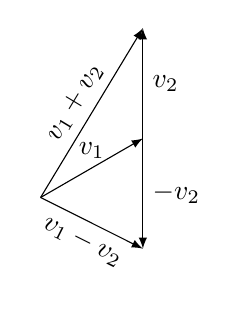
\begin{tikzpicture}
\pgfmathsetmacro{\da}{1.5}
\pgfmathsetmacro{\a}{30}
\pgfmathsetmacro{\db}{1.4}
\pgfmathsetmacro{\b}{90}
\draw[-latex](0,0)--++(\a:\da)coordinate(ka)node[pos=0.5,above]{$\kvec{v}_1$};
\draw[-latex](ka)--++(\b:\db)coordinate(kb)node[pos=0.5,right]{$\kvec{v}_2$};
\draw[-latex](ka)--++(-\b:\db)coordinate(kc)node[pos=0.5,right]{$-\kvec{v}_2$};
\draw[-latex](0,0)--(kb)node[pos=0.5,sloped, above]{$\kvec{v}_1+\kvec{v}_2$};
\draw[-latex](0,0)--(kc)node[pos=0.5,sloped,below]{$\kvec{v}_1-\kvec{v}_2$};
\end{tikzpicture}
\caption{سمتیات برائے سوال \حوالہ{سوال_سمتیہ_جیومیٹری_فرق_مجموعہ_الف}}
\label{شکل_سوال_سمتیہ_جیومیٹری_فرق_مجموعہ_الف}
\end{minipage}\hfill
\begin{minipage}{0.22\textwidth}
\centering
\begin{tikzpicture}
\pgfmathsetmacro{\r}{1.5}
\draw(0,0)node[circ]{}node[below]{$O$}circle (\r);
\draw[-latex](0,0)--(\r,0)node[right]{$B$}node[pos=0.5,below]{$\kvec{u}$};
\draw[-latex](0,0)--(-\r,0)node[left]{$A$}node[pos=0.5,below]{$-\kvec{u}$};
\draw[-latex](0,0)--++(140:\r)node[above]{$C$}node[pos=0.5,right]{$\kvec{v}$};
\end{tikzpicture}
\caption{دائرہ برائے سوال \حوالہ{سوال_سمتیہ_دائرہ_پر_نقطہ}}
\label{شکل_سوال_سمتیہ_دائرہ_پر_نقطہ}
\end{minipage}
\end{figure}

\ابتدا{سوال}
دکھائیں کہ یکساں اضلاع کے متوازی الاضلاع کے وتر ایک دوسرے کے عمودی ہوتے ہیں۔ 
\انتہا{سوال}
%========
\ابتدا{سوال}
دکھائیں کہ مربع وہ واحد مستطیل ہے جس کے وتر عمودی ہوتے ہیں۔
\انتہا{سوال}
%===============
\ابتدا{سوال}
ثابت کریں کہ ایک متوازی الاضلاع صرف اور صرف اس صورت مستطیل ہو گا جب اس کے وتروں  کی لمبائی ایک جیسی ہو۔ ترکھان اس حقیقت کو عموماً استعمال کرتا ہے۔
\انتہا{سوال}
%==========
\ابتدا{سوال}
متوازی الاضلاع کے قریبی ضلع \عددی{\kvec{u}} اور \عددی{\kvec{v}} ہیں۔ دکھائیں کہ ان کے مشترکہ راس سے مخالف راس تک وتر،  \عددی{\kvec{u}} اور \عددی{\kvec{v}} کے بیچ زاویہ کو دو برابر حصوں میں تقسیم کرتا ہے۔ 
\انتہا{سوال}
%=============
\ابتدا{سوال}
ایک اہرام کے مربع قاعدہ \عددی{OABC} کے ضلع  کی لمبائی \عددی{1} اکائی ہے  اور اہرام کی چوٹی \عددی{D} ہے۔اہرام کا قد بھی \عددی{1} اکائی ہے۔ یوں نقطہ  \عددی{D} ٹھیک وتر \عددی{OB} کے وسطی نقطہ کے سیدھا اوپر پایا جاتا ہے۔ قطع \عددی{\krightharpoonup{OB}} اور \عددی{\krightharpoonup{OD}} کے بیچ زاویہ تلاش کریں۔
\انتہا{سوال}
%===================
\ابتدا{سوال}\شناخت{سوال_سمتیہ_کوسائن_رخ}\ترچھا{زاویات رخ اور کوسائن رخ}\\
سمتیہ \عددی{\kvec{v}=a\ai+b\aj+c\ak} کے زاویات رخ \عددی{\alpha}، \عددی{\beta} اور \عددی{\gamma} کی تعریف درج ذیل ہے (شکل \حوالہ{شکل_سوال_سمتیہ_کوسائن_رخ})۔
\begin{enumerate}[]
\item
مثبت محور \عددی{x} اور \عددی{\kvec{v}} کے بیچ زاویہ \عددی{\alpha} ہے (\عددی{0\le\alpha\le\pi})،
\item
مثبت محور \عددی{y} اور \عددی{\kvec{v}} کے بیچ زاویہ \عددی{\beta} ہے (\عددی{0\le\beta\le\pi})،
\item
مثبت محور \عددی{z} اور \عددی{\kvec{v}} کے بیچ زاویہ \عددی{\gamma} ہے (\عددی{0\le\gamma\le\pi})۔
\end{enumerate}
\begin{enumerate}[a.]
\item
درج ذیل
\begin{align*}
\cos\alpha=\frac{a}{\abs{\kvec{v}}},\quad \cos\beta=\frac{b}{\abs{\kvec{v}}},\quad \cos\gamma=\frac{c}{\abs{\kvec{v}}}
\end{align*} 
اور \عددی{\cos^2\alpha+\cos^2\beta+\cos^2\gamma=1} دکھائیں۔ ان کوسائن کو \اصطلاح{کوسائن رخ}\فرہنگ{کوسائن!رخ}\حاشیہب{direction cosines}\فرہنگ{direction!cosines} کہتے ہیں۔
\item
\ترچھا{کوسائن رخ اور اکائی سمتیات۔} دکھائیں کہ اگر \عددی{\kvec{v}=a\ai+b\aj+c\ak} ایک اکائی سمتیہ ہو تب \عددی{a}، \عددی{b} اور \عددی{c} سمتیہ \عددی{\kvec{v}} کے کوسائن رخ ہوں گے۔
\end{enumerate}
\انتہا{سوال}
%======================
\begin{figure}
\centering
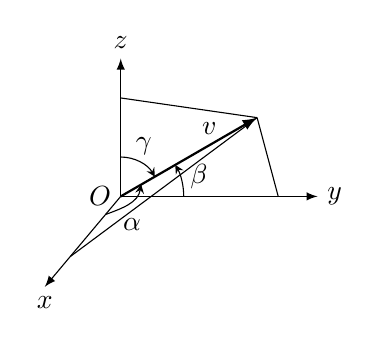
\begin{tikzpicture}
\pgfmathsetmacro{\len}{2}
\pgfmathsetmacro{\ang}{30}
\pgfmathsetmacro{\angX}{-130}
%\draw[-latex](0,0)node[left]{$O$}--(-1.25,-1.25)node[below]{$x$};
\draw[-latex](0,0)node[left]{$O$}--++(\angX:1.5)node[below]{$x$};
\draw[-latex](0,0)--(2.5,0)node[right]{$y$};
\draw[-latex](0,0)--(0,1.75)node[above]{$z$};
\draw[-latex,thick](0,0)--++(\ang:\len)coordinate(kt)node[pos=0.65,above]{$\kvec{v}$};
\draw(kt)--(2,0);
\draw(kt)--(0,1.25);
\draw(kt)--(\angX:1)coordinate(kk);
\RightAngle{(kt)}{(2,0)}{(0,0)}
\RightAngle{(kt)}{(0,1.25)}{(0,0)}
\RightAngle{(kt)}{(kk)}{(\angX:1.25)}
\draw[-stealth]([shift={(90:0.5)}]0,0) arc (90:\ang:0.5)node[pos=0.6,above]{$\gamma$};
\draw[-stealth]([shift={(0:0.8)}]0,0) arc (0:\ang:0.8)node[pos=0.6,right]{$\beta$};
\draw[-stealth](\angX:0.3) to [out=20,in=-100]node[pos=0.3,below,xshift=1ex]{$\alpha$}(\ang:0.3);
\end{tikzpicture}
\caption{زاویات رخ اور کوسائن رخ کی تعریف۔}
\label{شکل_سوال_سمتیہ_کوسائن_رخ}
\end{figure}

\موٹا{سمتیات کے بیچ زاویے}\\
سوال \حوالہ{سوال_سمتیہ_زاویات_بیچ_سمتیات_الف} تا سوال \حوالہ{سوال_سمتیہ_زاویات_بیچ_سمتیات_ب} میں کیلکولیٹر کی مدد سے سمتیات کے بیچ زاویات کو، ایک فی صد درست، ریڈیئن میں  تلاش کریں۔

\ابتدا{سوال}\شناخت{سوال_سمتیہ_زاویات_بیچ_سمتیات_الف}
$\kvec{A}=2\ai+\aj,\quad \kvec{B}=\ai+2\aj-\ak$
\انتہا{سوال}
%===================
\ابتدا{سوال}
$\kvec{A}=2\ai-2\aj+\ak,\quad \kvec{B}=3\ai+4\ak$
\انتہا{سوال}
%===================
\ابتدا{سوال}
$\kvec{A}\sqrt{3}\ai-7\aj,\quad \kvec{B}=\sqrt{3}\ai+\aj-2\ak$
\انتہا{سوال}
%===================
\ابتدا{سوال}\شناخت{سوال_سمتیہ_زاویات_بیچ_سمتیات_ب}
$\kvec{A}=\ai+\sqrt{2}\aj-\sqrt{2}\ak,\quad \kvec{B}=-\ai+\aj+\ak$
\انتہا{سوال}
%===================

سوال \حوالہ{سوال_سمتیہ_زاویات_بیچ_الف} تا سوال \حوالہ{سوال_سمتیہ_زاویات_بیچ_ب} میں کیلکولیٹر کی مدد سے سمتیات کے بیچ زاویات کو، ایک فی صد درست، ریڈیئن میں  تلاش کریں۔

\ابتدا{سوال}\شناخت{سوال_سمتیہ_زاویات_بیچ_الف}
مثلث \عددی{ABC} کے اندرونی زاویات۔ مثلث کے راس \عددی{A(-1,0,2)}، \عددی{B(2,1,-1)} اور \عددی{C(1,-2,2)} ہیں۔
\انتہا{سوال}
%=====================
\ابتدا{سوال}
سمتیات \عددی{\kvec{A}=2\ai+2\aj+\ak} اور \عددی{\kvec{B}=2\ai+10\aj-11\ak} کے بیچ زاویہ۔
\انتہا{سوال}
%====================
\ابتدا{سوال}\شناخت{سوال_سمتیہ_زاویات_بیچ_ب}
مکعب کے وتر اور مکعب کی ایک سطح کے وتر کے بیچ زاویہ۔ (اشارہ: ایسا مکعب استعمال کریں جس کے کنارے \عددی{\ai}، \عددی{\aj} اور \عددی{\ak} ہوں۔)
\انتہا{سوال}
%====================
\ابتدا{سوال}
پانی کی نالی میں ایک جوڑ ہے۔اس جوڑ سے  شمال رخ نالی کی ڈھلوان \عددی{\SI{10}{\percent}} ہے جبکہ جوڑ سے مشرق رخ نالی کی ڈھلوان \عددی{\SI{20}{\percent}} ہے۔ اس جوڑ پر نالی کے دو حصوں کے بیچ زاویہ کتنا ہو گا؟
\انتہا{سوال}
%==================

\موٹا{نظریہ اور مثالیں}\\
\ابتدا{سوال}
\begin{enumerate}[a.]
\item
کسی بھی سمتیات \عددی{\kvec{u}} اور \عددی{\kvec{v}} کے لئے عدم مساوات \عددی{\abs{\kvec{u}\cdot\kvec{v}}\le \abs{\kvec{u}}\abs{\kvec{v}}} کو \عددی{\kvec{u}\cdot\kvec{v}=\abs{\kvec{u}}\abs{\kvec{v}}\cos\theta} کی مدد سے دکھائیں۔
\item
کیا کبھی \عددی{\abs{\kvec{u}\cdot\kvec{v}}=\abs{\kvec{u}}\abs{\kvec{v}}} ہو سکتا ہے؟ اگر ہو سکتا ہے تب کب ایسا ہو گا؟  اپنے جواب کی وجہ پیش کریں۔
\end{enumerate}
\انتہا{سوال}
%=========
\ابتدا{سوال}
مستوی \عددی{xy} میں عمومی سمتیہ \عددی{\kvec{v}} بنائیں۔ اب ان نقطوں \عددی{(x,y)} کی نشاندہی کریں جن پر \عددی{(x\ai+y\aj)\cdot \kvec{v}=0} ہو گا۔ اپنے جواب کی وجہ پیش کریں۔
\انتہا{سوال}
%===============
\ابتدا{سوال}
اگر \عددی{\kvec{u}_1} اور \عددی{\kvec{u}_2} عمودی اکائی سمتیات ہوں اور \عددی{\kvec{v}=a\kvec{u}_1+b\kvec{u}_2} ہو تب \عددی{\kvec{v}\cdot\kvec{u}_1} تلاش کریں۔
\انتہا{سوال}
%===================
\ابتدا{سوال}\ترچھا{ضرب نقطہ میں مشترک اجزاء کی منسوخی}\\
حقیقی اعداد کے ضرب میں اگر \عددی{ab_1=ab_2} ہو اور \عددی{a} غیر صفر ہو تب دونوں اطراف \عددی{a} کو منسوخ کر کے \عددی{b_1=b_2} لکھا جا سکتا ہے۔ کیا ضرب نقطہ میں ایسا کرنا ممکن ہو گا: یعنی اگر \عددی{\kvec{A}\cdot\kvec{B}_1=\kvec{A}\cdot\kvec{B}_2} ہو تب کیا دونوں اطراف \عددی{\kvec{A}} منسوخ کر کے \عددی{\kvec{B}_1=\kvec{B}_2} لکھا جا سکتا ہے؟۔ اپنے جواب کی وجہ پیش کریں۔
\انتہا{سوال}
%====================
\ابتدا{سوال}
فرض کریں \عددی{\kvec{A}}، \عددی{\kvec{B}} اور \عددی{\kvec{C}} آپس میں عمودی سمتیات ہیں۔ اب \عددی{\kvec{D}=5\kvec{A}-6\kvec{B}+3\kvec{C}} لیں۔
\begin{enumerate}[a.]
\item
اگر \عددی{\kvec{A}}، \عددی{\kvec{B}} اور \عددی{\kvec{C}} اکائی سمتیات ہوں تب \عددی{\kvec{D}} کی مقدار \عددی{\abs{\kvec{D}}} تلاش کریں۔
\item
اگر \عددی{\abs{\kvec{A}}=2}، \عددی{\abs{\kvec{B}}=3} اور \عددی{\abs{\kvec{C}}=4} ہوں تب \عددی{\abs{\kvec{D}}} کتنا ہو گا؟
\end{enumerate}
\انتہا{سوال}
%==========
\ابتدا{سوال}
فرض کریں \عددی{\kvec{A}}، \عددی{\kvec{B}} اور \عددی{\kvec{C}} آپس میں عمودی اکائی سمتیات ہیں۔ اگر \عددی{\kvec{D}=\alpha\kvec{A}+\beta\kvec{B}+\gamma\kvec{C}} ہو جہاں \عددی{\alpha}، \عددی{\beta} اور \عددی{\gamma} غیر سمتی ہیں تب دکھائیں کہ \عددی{\alpha=\kvec{D}\cdot\kvec{A}}، \عددی{\beta=\kvec{D}\cdot\kvec{B}} اور \عددی{\gamma=\kvec{D}\cdot\kvec{C}} ہوں گے۔ 
\انتہا{سوال}
%===================

\موٹا{کام}\\
\ابتدا{سوال}
قوت \عددی{\kvec{F}=5\ak} (مقدار \عددی{5} نیوٹن) سیدھی لکیر پر مبدا سے نقطہ \عددی{(1,1,1)} تک  ایک جسم کو منتقل کرتا ہے (فاصلہ میٹر میں ہے)۔ یہ قوت کتنا کام کرتی ہے؟
\انتہا{سوال}
%============
\ابتدا{سوال}
ایک ریل گاڑی کا انجن \عددی{6000} ٹن کمیت کی ریل گاڑی کو \عددی{\SI{602148}{\newton}} قوت سے کھینچ سکتا ہے۔ ایک افقی سیدھی پٹڑی پر \عددی{605} کلو میٹر فاصلہ طے کر کے یہ انجن کتنا کام کرتا ہے؟
\انتہا{سوال}
%======================
\ابتدا{سوال}
ایک بوجھ کو \عددی{\SI{20}{\meter}} لمبی ڈھلوان پر \عددی{\SI{200}{\newton}} قوت کھینچتی ہے۔افقی سطح کے ساتھ یہ قوت \عددی{30^{\circ}} کا زاویہ بناتی ہے۔ یہ قوت کتنا کام کرتی ہے؟ 
\انتہا{سوال}
%================
\ابتدا{سوال}
ایک کشتی کے  بادبان پر ہوا \عددی{\SI{2000}{\newton}} قوت لگاتی ہے۔ افقی سطح کے ساتھ قوت کا زاویہ \عددی{60^{\circ}} ہے۔ ایک کلومیٹر فاصل طے کرنے میں یہ قوت کتنا کام کرتی ہے؟
\انتہا{سوال}
%===================

\موٹا{مستوی میں خط کی مساواتیں}\\
\ابتدا{سوال}\شناخت{سوال_سمتیہ_لکیر_عمودی_سمتیہ}
دکھائیں کہ سمتیہ \عددی{\kvec{v}=a\ai+b\aj} لکیر \عددی{ax+by=c} کو عمودی ہے۔ ایسا کرنے کی خاطر دکھائیں کہ اس لکیر کی ڈھلوان، اس سمتیہ کی ڈھلوان کے بالعکس متناسب کا نفی ہے۔
\انتہا{سوال}
%==========================
\ابتدا{سوال}\شناخت{سوال_سمتیہ_لکیر_متوازی_سمتیہ}
دکھائی کہ سمتیہ \عددی{\kvec{v}=a\ai+b\aj} لکیر \عددی{bx-ay=c} کے متوازی ہے۔ ایسا کرنے کی خاطر دکھائیں کہ لکیر کی ڈھلوان اور سمتیہ کی ڈھلوان ایک دوسرے جیسے  ہیں۔
\انتہا{سوال}
%====================

سوال \حوالہ{سوال_سمتیہ_عمودی_خط_الف} تا سوال \حوالہ{سوال_سمتیہ_عمودی_خط_ب} میں سوال \حوالہ{سوال_سمتیہ_لکیر_عمودی_سمتیہ} کا نتیجہ استعمال کر کے نقطہ \عددی{N} پر  \عددی{\kvec{v}} کے عمودی خط کی مساوات دریافت کریں۔ اس لکیر کو ترسیم کر کے مبدا پر اس عمودی سمتیہ کا بھی خاکہ بنائیں۔

\ابتدا{سوال}\شناخت{سوال_سمتیہ_عمودی_خط_الف}
$N(2,1),\quad \kvec{v}=\ai+2\aj$
\انتہا{سوال}
%====================== 
\ابتدا{سوال}
$N(-1,2),\quad \kvec{v}=-2\ai-\aj$
\انتہا{سوال}
%====================== 
\ابتدا{سوال}
$N(-2,-7),\quad \kvec{v}=-2\ai+\aj$
\انتہا{سوال}
%====================== 
\ابتدا{سوال}\شناخت{سوال_سمتیہ_عمودی_خط_ب}
$N(11,10),\quad \kvec{v}=2\ai-3\aj$
\انتہا{سوال}
%====================== 


سوال \حوالہ{سوال_سمتیہ_متوازی_خط_الف} تا سوال \حوالہ{سوال_سمتیہ_متوازی_خط_ب} میں سوال \حوالہ{سوال_سمتیہ_لکیر_متوازی_سمتیہ} کا نتیجہ استعمال کر کے نقطہ \عددی{N} پر  \عددی{\kvec{v}} کے متوازی خط کی مساوات دریافت کریں۔ اس لکیر کو ترسیم کر کے مبدا پر اس متوازی سمتیہ کا بھی خاکہ بنائیں۔

\ابتدا{سوال}\شناخت{سوال_سمتیہ_متوازی_خط_الف}
$N(-2,1),\quad \kvec{v}=\ai-\aj$
\انتہا{سوال}
%=========================
\ابتدا{سوال}
$N(0,-2),\quad \kvec{v}=2\ai+3\aj$
\انتہا{سوال}
%=========================
\ابتدا{سوال}
$N(1,2),\quad \kvec{v}=-\ai-2\aj$
\انتہا{سوال}
%=========================
\ابتدا{سوال}\شناخت{سوال_سمتیہ_متوازی_خط_ب}
$N(1,3),\quad \kvec{v}=3\ai-2\aj$
\انتہا{سوال}
%=========================

\موٹا{مستوی میں خطوط کے بیچ زاویے}\\
دو مستوی خط جن کے بیچ زاویہ حادہ جو قائمہ نہ ہو  وہی ہو گا جو ان خطوط کے عمودی دو سمتیات کے بیچ یا ان خطوط کے متوازی دو سمتیات کے بیچ ہو گا۔اس حقیقت کے ساتھ  سوال \حوالہ{سوال_سمتیہ_لکیر_عمودی_سمتیہ} یا سوال \حوالہ{سوال_سمتیہ_لکیر_متوازی_سمتیہ} کا نتیجہ استعمال کرتے ہوئے  سوال \حوالہ{سوال_سمتیہ_تلاش_زاویہ_الف} تا سوال \حوالہ{سوال_سمتیہ_تلاش_زاویہ_ب} میں خطوط کے بیچ زاویہ تلاش کریں۔

\ابتدا{سوال}\شناخت{سوال_سمتیہ_تلاش_زاویہ_الف}
$3x+y=5,\quad 2x-y=4$
\انتہا{سوال}
%=====================
\ابتدا{سوال}
$y=\sqrt{3}x-1,\quad y=-\sqrt{3}x+2$
\انتہا{سوال}
%=====================
\ابتدا{سوال}
$\sqrt{3}x-y=-2,\quad x-\sqrt{3}y=1$
\انتہا{سوال}
%=====================
\ابتدا{سوال}\شناخت{سوال_سمتیہ_تلاش_زاویہ_ب}
$x+\sqrt{3}y=1,\quad (1-\sqrt{3})x+(1+\sqrt{3})y=8$
\انتہا{سوال}
%=====================

سوال \حوالہ{سوال_سمتیہ_زاویہ_خط_الف} اور سوال \حوالہ{سوال_سمتیہ_زاویہ_خط_ب} میں خطوط کے بیچ  ایک ریڈیئن کے سواں حصہ تک زاویہ حادہ تلاش کریں۔

\ابتدا{سوال}\شناخت{سوال_سمتیہ_زاویہ_خط_الف}
$3x-4y=3,\quad x-y=7$
\انتہا{سوال}
%=====================
\ابتدا{سوال}\شناخت{سوال_سمتیہ_زاویہ_خط_ب}
$12x+5y=1,\quad 2x-2y=3$
\انتہا{سوال}
%=====================

\موٹا{قابل تفرق منحنیات کے بیچ زاویہ}\\
دو قابل تفرق منحنیات کے نقطہ تقاطع پر ان کے بیچ زاویہ سے مراد اس نقطہ پر منحنیات کے مماس کے بیچ زاویہ ہے۔ سوال \حوالہ{سوال_سمتیہ_بیچ_زاویہ_الف} تا سوال \حوالہ{سوال_سمتیہ_بیچ_زاویہ_ب} میں منحنیات کے بیچ زاویات دو نقاط تقاطع پر معلوم کریں۔  (آپ کو کیلکولیٹر کی ضرورت پیش نہیں آئے گی۔)

\ابتدا{سوال}\شناخت{سوال_سمتیہ_بیچ_زاویہ_الف}
$y=\tfrac{3}{2}-x^2,\quad y=x^2$
\انتہا{سوال}
%=======================
\ابتدا{سوال}
$x=\tfrac{3}{4}-y^2,\quad x=y^2-\tfrac{3}{4}$
\انتہا{سوال}
%======================
\ابتدا{سوال}
$y=x^3,\quad x=y^2$
\انتہا{سوال}
%======================
\ابتدا{سوال}\شناخت{سوال_سمتیہ_بیچ_زاویہ_ب}
$y=-x^2,\quad y=\sqrt[3]{x}$
\انتہا{سوال}
%======================
